% -*- Mode:TeX -*-
% TODO Try using ACM SIGCHI two-column layout
% TODO Need to make sure verb tense is consistent. Sometimes I use future and sometimes present.

%% The documentclass options along with the pagestyle can be used to generate
%% a technical report, a draft copy, or a regular thesis.  You may need to
%% re-specify the pagestyle after you \include cover.tex.  For more
%% information, see the first few lines of mitthesis.cls.

\documentclass{chi2011}
\usepackage{times}
%\copyrightnotice{This work is licensed under a Creative Commons Attribution 3.0 Unported License}
\usepackage{graphicx}
\usepackage{ucs}
\usepackage[utf8x]{inputenc}
\usepackage[pdftex]{hyperref}
\usepackage{color}

\hypersetup{%
pdftitle={Designing for Remixing: Supporting an Online Community of Amateur Creators},
pdfauthor={Andres Monroy-Hernandez},
pdfkeywords={remixing, online communities},
bookmarksnumbered,
pdfstartview={FitH},
colorlinks,
citecolor=black,
filecolor=black,
linkcolor=black,
urlcolor=black,
breaklinks=true,
}
\newcommand{\comment}[1]{}
\definecolor{Orange}{rgb}{1,0.5,0}
\newcommand{\todo}[1]{\textsf{\textbf{\textcolor{Orange}{[[#1]]}}}}

\pagenumbering{arabic}  % Arabic page numbers for submission.  Remove this line to eliminate page numbers for the camera ready copy

% add bibliographic stuff 
\usepackage[round]{natbib}
%%Prefatory material
\bibliographystyle{apalike}
%\bibliographystyle{acmnocaps}
%\bibliographystyle{acm-sigchi}
\def\citepos#1{\citeauthor{#1}'s (\citeyear{#1})}
\def\citespos#1{\citeauthor{#1}' (\citeyear{#1})}

%% This bit allows you to either specify only the files which you wish to
%% process, or `all' to process all files which you \include.
%% Krishna Sethuraman (1990).

% andresmh: commenting this out will ask you to manually enter which files you need to compile
%\typein [\files]{main}
%\ifx\files\blank \typeout{Including all files.} \else \typeout{Including only \files.} \includeonly{\files} \fi

\begin{document}
\special{papersize=8.5in,11in}
\setlength{\paperheight}{11in}
\setlength{\paperwidth}{8.5in}
\setlength{\pdfpageheight}{\paperheight}
\setlength{\pdfpagewidth}{\paperwidth}
\toappear{Thesis proposal submitted to the Program in Media Arts and Sciences, School of Architecture and Planning, in partial fulfillment of the requirements for the degree of Doctor of Philosophy in Media Arts and Sciences. \\This work is licensed under a Creative Commons. Attribution 3.0 Unported License} 
%%Formatting commands
%\setlength{\parindent}{0pt} %Full block style
%\setlength{\parskip}{11pt} %Assumes 11pt type
\hfuzz2pt % Don't bother to report over-full boxes if over-edge is < 2pt
%%Prefatory material
%\bibliographystyle{apalike}
%\bibliographystyle{acm-sigchi}
% -*-latex-*-
% $Log: cover.tex,v $
% Revision 1.6  1999/10/21 14:49:31  boojum
% changed comment referring to documentstyle
%
% Revision 1.5  1999/10/21 14:39:04  boojum
% *** empty log message ***
%
% Revision 1.4  1997/04/18  17:54:10  othomas
% added page numbers on abstract and cover, and made 1 abstract
% page the default rather than 2.  (anne hunter tells me this
% is the new institute standard.)
%
% Revision 1.4  1997/04/18  17:54:10  othomas
% added page numbers on abstract and cover, and made 1 abstract
% page the default rather than 2.  (anne hunter tells me this
% is the new institute standard.)
%
% Revision 1.3  93/05/17  17:06:29  starflt
% Added acknowledgements section (suggested by tompalka)
%
% Revision 1.2  92/04/22  13:13:13  epeisach
% Fixes for 1991 course 6 requirements
% Phrase "and to grant others the right to do so" has been added to
% permission clause
% Second copy of abstract is not counted as separate pages so numbering works
% out
%
% Revision 1.1  92/04/22  13:08:20  epeisach
\title{Designing for Remixing:\\Supporting an Online Community of Amateur Creators}
\numberofauthors{1}
\author{
  \alignauthor Andrés Monroy-Hernández\\
%  \affaddr{Massachusetts Institute of Technology, Cambridge, MA 02139}\\
%  \email{amonroy@mit.edu}
}

%\prevdegrees{S.M., Massachusetts Institute of Technology (2007) \\B.S., Tecnológico de Monterrey (2001)}
%\department{Program in Media Arts and Sciences}
%\school{School of Architecture and Planning}
% If the thesis is for two degrees simultaneously, list them both
% separated by \and like this:
% \degree{Doctor of Philosophy \and Master of Science}
%\degree{Doctor of Philosophy in Media Arts and Sciences}
%\degreemonth{April}
%\degreeyear{2011}
%\thesisdate{May 6, 2011}

%% By default, the thesis will be copyrighted to MIT.  If you need to copyright
%% the thesis to yourself, just specify the `vi' documentclass option.  If for
%% some reason you want to exactly specify the copyright notice text, you can
%% use the \copyrightnoticetext command.
%\copyrightnoticetext{\copyright IBM, 1990.  Do not open till Xmas.}

% If there is more than one supervisor, use the \supervisor command
% once for each.
%\supervisor{Mitchel Resnick}{LEGO Papert Professor of Learning Research}{MIT Media Laboratory}

% This is the department committee chairman, not the thesis committee
% chairman.  You should replace this with your Department's Committee
% Chairman.
%\chairman{Foo Bar}{Chair, Departmental Committee on Graduate Students}{Program in Media Arts and Sciences}

% Make the titlepage based on the above information.  If you need
% something special and can't use the standard form, you can specify
% the exact text of the titlepage yourself.  Put it in a titlepage
% environment and leave blank lines where you want vertical space.
% The spaces will be adjusted to fill the entire page.  The dotted
% lines for the signatures are made with the \signature command.
\maketitle

%%%%%%%%%%%%%%%%%%%%%%%%%%%%%%%%%%%%%%%%%%%%%%%%%%%%%%%%%%%%%%%%%%%%%%
% -*-latex-*-
%\cleardoublepage

%abstract.tex
%Abstract for AYB PhD thesis

% The abstractpage environment sets up everything on the page except
% the text itself.  The title and other header material are put at the
% top of the page, and the supervisors are listed at the bottom.  A
% new page is begun both before and after.  Of course, an abstract may
% be more than one page itself.  If you need more control over the
% format of the page, you can use the abstract environment, which puts
% the word "Abstract" at the beginning and single spaces its text.

%% You can either \input (*not* \include) your abstract file, or you can put
%% the text of the abstract directly between the \begin{abstractpage} and
%% \end{abstractpage} commands.

% First copy: start a new page, and save the page number.
%\cleardoublepage
% Uncomment the next line if you do NOT want a page number on your
% abstract page.
% \pagestyle{empty}
%\setcounter{savepage}{\thepage}
\begin{abstract}
%\addcontentsline{toc}{chapter}{Abstract}
%\setlength{\parskip}{0pt} %Assumes 11pt type
%\begin{spacing}{1}
In this dissertation proposal I describe a framework to design and study an online community of amateur creators.
I focus on remixing as the lens to understand the social, cultural and technical infrastructure of a social media environment that supports creative expression.
I am motivated by three broad questions:
1) what are the \emph{structural} properties of an online remixing community?
2) what is the \emph{functional} role of remixing in cultural production and social learning?
3) what are amateur creators' \emph{attitudes} towards remixing?
As part of this work, I conceived, developed and studied the Scratch Online Community: a website where young people share and remix their own video games and animations, as well as those of their peers.
In three years, the community has grown to close to 800,000 registered members and more than 1.7 million community-contributed projects.
%\end{spacing}
%\setlength{\parskip}{11pt plus3pt minus3pt} %Assumes 11pt type
\end{abstract}

%\cleardoublepage

%\keywords{put author keywords here} 
%\category{H.5.2}{Information Interfaces and Presentation}{Miscellaneous}[Optional sub-category]
%\terms{
%  See list of the limited ACM 16 terms in the instructions, see http://www.sheridanprinting.com/sigchi/generalterms.htm.
%}
%%readers.tex
%Readers page for AYB PhD thesis

% Provides a signature page for secondary readers on a thesis. Title info
% is gathered from the title page, and readers can be added below.
% Media Lab requires this. [AYB]
\reader{Yochai Benkler}{Berkman Professor of Entrepreneurial Legal Studies}{Harvard University}
\reader{Robert C. Miller}{Associate Professor of Computer Science of Electrical Engineering and Computer Science}{MIT Computer Science and Artificial Intelligence Laboratory}

\readerpage

%\cleardoublepage

%\pagestyle{plain}
%%Main body (chapters)
%\setlength{\parskip}{0pt} %Assumes 11pt type
%\begin{spacing}{1}
%  % -*- Mode:TeX -*-
%% This file simply contains the commands that actually generate the table of
%% contents and lists of figures and tables.  You can omit any or all of
%% these files by simply taking out the appropriate command.  For more
%% information on these files, see appendix C.3.3 of the LaTeX manual.

\tableofcontents
%\newpage
%\listoffigures
%\newpage
%\listoftables

%\end{spacing}
%\setlength{\parskip}{11pt plus3pt minus3pt} %Assumes 11pt type
\chapter{Introduction}

\chapter{Background}

Remixes, mash-ups, forks and derivative works are terms used to refer to a form of social production based on the idea of creating something out of existing creations.
From Wikipedians editing each other's articles, to Free and Open Source programmers reusing existing code libriaries, to teenagers mixing their favorite videos on YouTube, are all examples of the wide range of remixing practices found today in the digital landscape.

% TODO: add more references about the intersection of community and remixing
I build on existing work that places remixing in new forms of economic and cultural production \citep{benkler_wealth_2006,jenkins_convergence_2006,manovich_remix_2005,sinnreich_ethics_2009}, and describes some challenges that remixing poses to our existing legal and moral assumptions \citep{lessig_remix:_2008, posner_little_2007}.

% SELF: My work will build more on new media literacy than on situated learning so I am mentioning this first.
Furthermore, I build on work that advocates remixing as a new media literacy skill \citep{ito_hanging_2010, jenkins_confronting_2009, livingstone_taking_2008, perkel_copy_2008} and that positions remixing as legitimate form of participation in social learning environments, building on learning philosophies such as Constructionism \citep{papert_mindstorms_1980} and Situated Learning \citep{lave_situated_1991}.

Finally, I look at the implications of remixing for the design of social computing systems. I do this by connecting to research on human-computer interaction that examines the participation patterns and the design of peer-production communities that engage people in sharing and remixing videos \citep{diakopoulos_evolution_2007,shaw_community_2006}, images \citep{seneviratne_policy-aware_2009}, music \citep{cheliotis_analysis_2009} and hypertext \citep{viegas_studying_2004}.

\section{Economic and Cultural Production}

Network information technologies have enabled social production to emerge as a new form of economic production, in parallel to markets and firms.
People engaging in this new form of production, referred to as Commons-based Peer Production \citep{benkler_coases_2002}, rely on the availability of existing common resources that are often repurposed for the creation of new products that end up going back that communal source, for others to reuse as well.

Culture has also been influenced by these new forms of peer-to-peer participation where the boundaries between producers and consumers blur, what \citet{jenkins_convergence_2006} calls Participatory Culture.

This seemingly new creative practices, based on the idea of building new things by combining existing ones, is not necessarily new. 
Artists, especially postmodernist, have engaged in similar practices through ``appropriation art'', ``pastiche'', ``collage'', ``sampling'' and ``bricolage''. 
Furthermore, folk culture and oral traditions very much rely on this idea of recreating and remixing what others have made. %Citation need
For example, as \citet{manovich_remix_2005} argues, remixing is an integral part of cultural evolution as one can see how ancient Rome was a remix of ancient Greece.
Despite this common feeling that everything old is new again, the influence of digital technologies in remixing-like practices is undeniable. 
These technologies have enabled people to a) create perfect copies and b) go beyond just being able to be inspired by other's creations but to actually remix the original works themselves \citep{sinnreich_ethics_2009}.

\section{Learning and New Media Literacy}

Remixing is a social activity by nature. Hence, some of the discussions around remixing and learning stem from learning theories that look at the social context in which learning happens.
Situated Learning is one of these models that has advocated for legitimizing peripheral forms of participation, in particular in the context of apprenticeship-like learning environments \citep{lave_situated_1991}. 
This apprenticeship model is also central to Constructionism \citep{papert_mindstorms_1980}, a learning philosophy based on the idea that some of the most valuable learning experiences occur when children engage in building personally meaningful objects in a social context. 
% TODO: Look at how Bruckman cites this in the social context
% NOTE: I'll move this next sentence to Scratch Online Community: Motivations
% In examining, apprenticeships as a valuable learning model, \citet{papert_mindstorms_1980} uses as the example of the Brazilian Samba schools. These schools allow both novices and experts to learn from each other by building on each others work and expertise in an ad-hoc fashion.
Building on this theory, \citet{turkle_epistemological_1990} argued for ``bricolage'' as a legitimate learning style, alternative to planning, where learners ``construct theories by arranging and rearranging, by negotiating and renegotiating with a set of well-known materials'', a model that fits well with the process of remixing.

Similarly, \citet{wenger_communities_1998} stressed the importance of also having access to a ``shared repertoire of communal resources'' to help shape a ``community of practice.''

More recently, cultural anthropologists and media scholars have documented the ways young people engage in creative practices through remixing. 
For example, \citet{ito_technologies_2007} described how children relate to media franchises, such as Pókemon.
She found that children not only consume Pókemon but they actively engage in remixing and recreating it, ``demonstrating that children can master highly esoteric content, customization, connoisseurship, remixing.''
\citet{livingstone_taking_2008} has described similar practices when it comes to Internet usage and presented the challenges and possibilities that these creative practices promise.
Similarly, \citet{jenkins_convergence_2006} has narrated how kids have become active participants in media creation by remixing their favorite literary characters in Harry Potter and creating rich fan fiction.
Later on, \citet{jenkins_confronting_2009} argued that the ability to remix, is a core competency that children must possess in order to be fluent with new media.

\section{Ethical and Legal Challenges}

Creative appropriation or remixing has been confronted on moral and legal grounds.
In his description children's fan fiction, \citet{jenkins_convergence_2006} narrates how the young girl who created an Harry Potter fan fiction website, was challenged by the company who owns the legal rights to book and the movie, on the grounds of copyright infringement.
Realizing of their copyright extremism, the company dropped the legal action and reached an agreement.

More recently, appropriation art has been under legal scrutiny \citep{greenberg_art_1992,landes_copyright_2000}. 
For example, a federal court judge determined that photographer Richard Price violated Patrick Cariou’s copyrights for remixing a set of pictures by putting them on frames and in some cases, ``painting over some portions'' \citep{batts_patrick_2011}.

Similarly, countless number of video remixes on video sharing website YouTube have been taken down under the Digital Millenium Copyright Act, for being identified as remixes of commercial videos \citep{seneviratne_remix_2010}.

\citet{posner_little_2007} has articulated how plagiarism is highly context-dependent but that one can assess the ethics of appropriation by thinking through issues of deception, perception and social expectation.
\citet{benkler_wealth_2006} argues that if we want peer-production to flourish, we must figure out how to enable remixing:
``If we are to make this culture our own, render it legible, and make it into a new platform for our needs and conversations today, we must find a way to cut, paste, and remix present culture. And it is precisely this freedom that most directly challenges the laws written for the twentieth-century technology, economy, and cultural practice.''

Similarly, \citet{lessig_remix:_2008} has narrated the cases of ``copyright extremism'' that, he argues, ``chill''
 innovation and creativity, especially among young people who often engage in this practices.
In response to such copyright extremism, the Creative Commons licenses, to allow creators have more control of their copyright and release their work under more permissive licenses that would foster amateur creativity.

At the core of the ethics of remixing lies the issue of human cooperation, that is, the idea of how much people are willing to sacrifice their selfish and rational desires, to obtain monetary or reputation gains, to behave in altruistic and cooperative ways. 
These questions lay at the core of literature on human cooperation which is beginning to be translated to social system design.

\section{Social Computing System Design}

Human-computer interaction research has studied the use and design of social computer systems that foster the type of cooperative practices that allow for remixing to take place.
% Wikipedia
Wikipedia has been perhaps the most widely researched of those systems. 
For example, \citet{viegas_studying_2004} developed a visualization of Wikipedia edits that led to insights on the nature of the system and its editors' ability to collaborate. 
Later on \citet{kittur_harnessing_2008} studied Wikipedia's articles quality in relationship with different types of coordination mechanisms.
% Open Source
Similarly, analyses on open source software development have led to insights at the mechanisms that lead to successful cooperative projects. 
\citet{raymond_cathedral_1999}, for example, argued that one of the lessons to be learned from open source software programmers, is the importance of knowing what to rewrite and reuse. 
He describes how Linus Trovalds (the creator of Linux) did not ``try to write Linux from scratch'' but rather ``he started by reusing code and ideas from Minix, a tiny Unix-like OS for PC clones.'' 

% Tools
Researchers have also developed web mash-up tools that allow people to remix web content \citep{bolin_automation_2005,wong_making_2007}.
A study on one of those web mash-up tools found that many of its users lacked programming skills and found web mash-up to be a effective way of searching and aggregating information \citet{nan_zang_whats_2008}.

% Media sharing and remixing commmunities
More specifically on online communities for remixing, \citet{shaw_community_2006} developed a video remixing platform and studied the nature of the most generative video segments looking to understand how to integrate automatic recommendation systems with user-driven suggestions.
\citet{diakopoulos_evolution_2007} analyzed user's participation in a video remixing website and documented how participants developed certain norms for appropriating other people's work that were not encoded in the architecture of the website.
Additionally, a study of the music remixing online community ccMixter.org, looked at the impact of a remixing contest in the community dynamics.
The study found that the contests increased participation among new comers but that they did not continue using the website after the contest was over \citep{cheliotis_analysis_2009}. 


\chapter{The Scratch Online Community}

%TODO: once settled with layout, make sure it does not use a full page just for this image
\begin{figure}
\centering
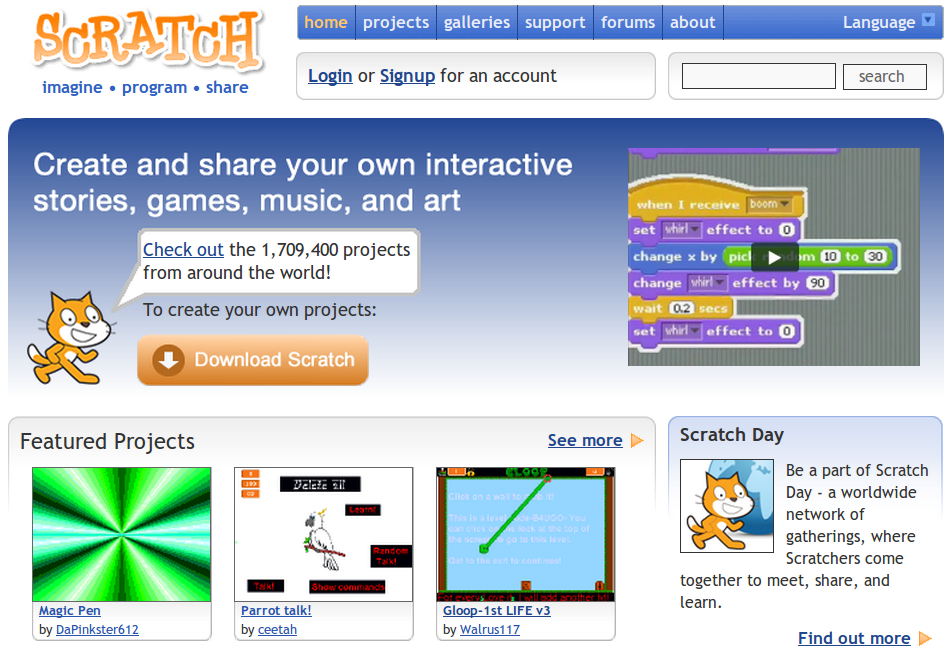
\includegraphics[width=3.25in]{figures/websitehomepage.png}
\caption{The home page of the Scratch website}
\label{fig:websitehomepage}
\end{figure}

The empirical setting for this work is the Scratch Online Community, a website (Figure~\ref{fig:websitehomepage}) I conceived and developed over the past four years, for this and other lines of research.
The website allows anyone, especially young people between ages eight and sixteen, to share their animated stories, interactive art, and video games. Participants use the Scratch programming environment to create or remix projects by putting together images, music and sounds with programming command blocks \citep{resnick_scratch:_2009}.
Projects range from interactive greeting cards, physics simulations, animations of popular songs to homemade video games, just to name a few.  

In my dissertation, I plan to document in detail the motivations that led to the design of the Scratch website as it is now and the various iterations that it went through as a result of internal and user-driven demands and participation patterns.
I expand on the tight relationship between the technical capabilities of the website and the social dynamics that it supported or intended to support.
I take a critical look at how the original goals of the community were or were not achieved and in what ways that happened. 
I narrate scalability challenges with the technology and moderation of the community.
In the following two sections I provide a glimpse of this.

More broadly, I try to tackle questions such as: How the culture of sharing was seeded and maintained in a public space? What were some important incidents that changed policies or architecture? How the architecture and management of the site influenced the culture of the site and how users helped shaped this? 
Was it the design of the space or the work of users to create the culture?
 What were the lessons learned along the way by administrators? What kinds of learning outcomes were achieved?
To answer some of these questions, I primarily rely on participant observation data, experiences collected during the three years and I support these arguments with descriptive statistics and case studies.


\section{Motivations}

From its start \citep{monroy-hernandez_scratchr:_2007,monroy-hernandez_empowering_2008}, I set the goal for the Scratch Online Community as to give creators access to 
1) a \emph{network of peers} that functions as an audience and as potential collaborators and,
2) a \emph{repository} of inspirational creations that can be creatively appropriated by anyone.

More broadly, the Scratch Online Community was created with the idea of supporting a Community of Practice around Scratch where novices and experts would come together,  in the spirit of Papert's Samba school's metaphor \citep{papert_mindstorms_1980}.

Additionally, the idea of the Scratch Online Community was conceived under the umbrella of embodying the ethos of Participatory Culture of empowering people to become producers rather than just consumers of media.

Last, the Scratch Online Community was motivated to support the various iterative stages of the creative process \citep{resnick_sowing_2008}, namely:
Supporting creators' \emph{imagination} by giving access to a pool of inspirational projects and ideas; supporting \emph{creation} by allowing people to reuse and remix; supporting \emph{play} by letting people interact with others and their creations within a community; supporting \emph{sharing} by allowing people to easily upload their creations to the platform; supporting \emph{reflection} by providing a space to receive comments and discussion forums for more in-depth discussions.

\section{Sociotechnical Infrastructure}
The Scratch website platform, called ScratchR, is broadly composed of the following components: 

\begin{enumerate}
\item A repository of projects and metadata. Projects can be downloaded by anyone, modified and re-uploaded to the website as a remix. Each project has its web page where it is displayed and where people can interact with it and other people. Projects themselves are created in Scratch, a desktop application people download and install on their computers. Projects are created by putting together images, sounds and visual programming blocks. Projects are organized in sprites (e.g. a character in a game). Each sprite has a set of ``costumes'' or images that represent the different its different visual states, for example, a sprite of a bird flying could have multiple costumes, each one representing the different positions of the wings. Sprites can also have sounds associated to them, these sounds can be either recorded with the microphone or imported from the hard creator's hard drive. Finally, sprites' behavior is controlled by ``scripts'' which are stacks of visual programming blocks. 

\item A social network consisting of profile pages and unidirectional friendship connections. Profile pages list the friends, projects and ``favorited'' projects for each user with his or her avatar image and the Country of origin (all self-reported data).

\item Social features for interacting with people's creation such as commenting, tagging, ``loving'', ``favoriting''.

\item Galleries, which are pages where people can group projects and talk about them. It is important to note that galleries have been repurposed by the community as group spaces where people collaborate to create projects or use it as a space to talk to one another or play Role Playing Games.

\item Discussion forums where community members help one another with technical problems, find collaborators and talk about non-Scratch related activities that foster a sense of community on the website.

\item External services supported by APIs such as a website where people can link projects or a Wiki where people can document their experiences with Scratch and the community.
\end{enumerate}

The website runs on a hybrid model for moderation that combines user-driven moderation through flagging and appointed moderators working in parallel with a full-time staff member and other part-time ones that review the flags and ensure that the social dynamics are kept as civil as possible. 
This model has allowed for scaling the community management at a relatively low cost, however, much of the architecture and software development during the three years has been put into mechanisms for preventing antisocial behavior.

Three years after its official release, the Scratch Online Community website I developed, handles more than ten million page views and six hundred-thousand people monthly.
This web traffic is more than half the page views of websites like newsweek.com \footnote{04/2011 data from http://www.quantcast.com/newsweek.com} and one-third of a website like economist.com \footnote{04/2011 data from http://http://www.quantcast.com/economist.com}.
As of April of 2011, more than 1.7 million projects have been uploaded at an average of 1 MB per project. 
Every second, the website receives up to 180 requests and it transfers 4MB.

To handle this level of activity, ScratchR, the website's underlying platform, uses a caching engine for static content called Varnish and another for dynamic content and database queries called Memcached. 
ScratchR runs on a completely Free and Open Source software stack that includes Apache for its web server and MySQL for its database running on CentOS Linux. 
ScratchR is written using a PHP-based framework called CakePHP.
Additionally, the ScratchR supports external  web applications such as a discussion forum, a user-driven Wiki, a statistics visualization website, a Scratch sprites sharing website, and few other websites that provide additional support to community members. 
These extra websites are supported through an API\footnote{API stands for Application Program Interface. In ScratchR, they are a set of web-accesible functions accessible via web that let people retrieve and submit data such as login authentication and information about projects.} that has allowed scalability.

\section{Research}

I propose a framework to examine remixing in an online community of amateur creators. 
I approach this by first studying the design of the online community as a remixing system, and then analyzing what people do and how they react to what others do.
More specifically, I focus on the structural, functional and attitudinal characteristics of an online community's sociotechnical infrastructure and its participants activities.
This framework derives from and is examined through design interventions, three-years of participant observation data, case studies, interviews with community members, quantitative and network analysis of a large corpus of data that includes more than 700,000 registered accounts and a repository of more than 9 million comments and 1.6 million interactive media objects, 30\% of which are remixes.

\section{Structure of a Remixing System} 
I plan to study the sociotechnical architecture of the Scratch Online Community by examining its following structural attributes (Figure~\ref{fig:structure}):
1) granularity of the remixable components, 
2) modularity of the remixable components, 
3) decomposability of finished projects, 
4) attributability mechanisms and 
5) openness to remix across systems.

In this proposal I briefly define each structural attribute using one or two examples and I explain how I am planning to go about studying it.
I plan to do analyze these structural properties of the system using varied approaches including:
1) case studies that give an rich description of different scenarios that elucidate on the influence of each attribute,
2) analyses the data corpus to understand the frequency of the scenarios and the relationships between the structural attributes,
3) natural design experiments to study the effect of varying some of the structural dimensions.

\begin{figure} 
\centering
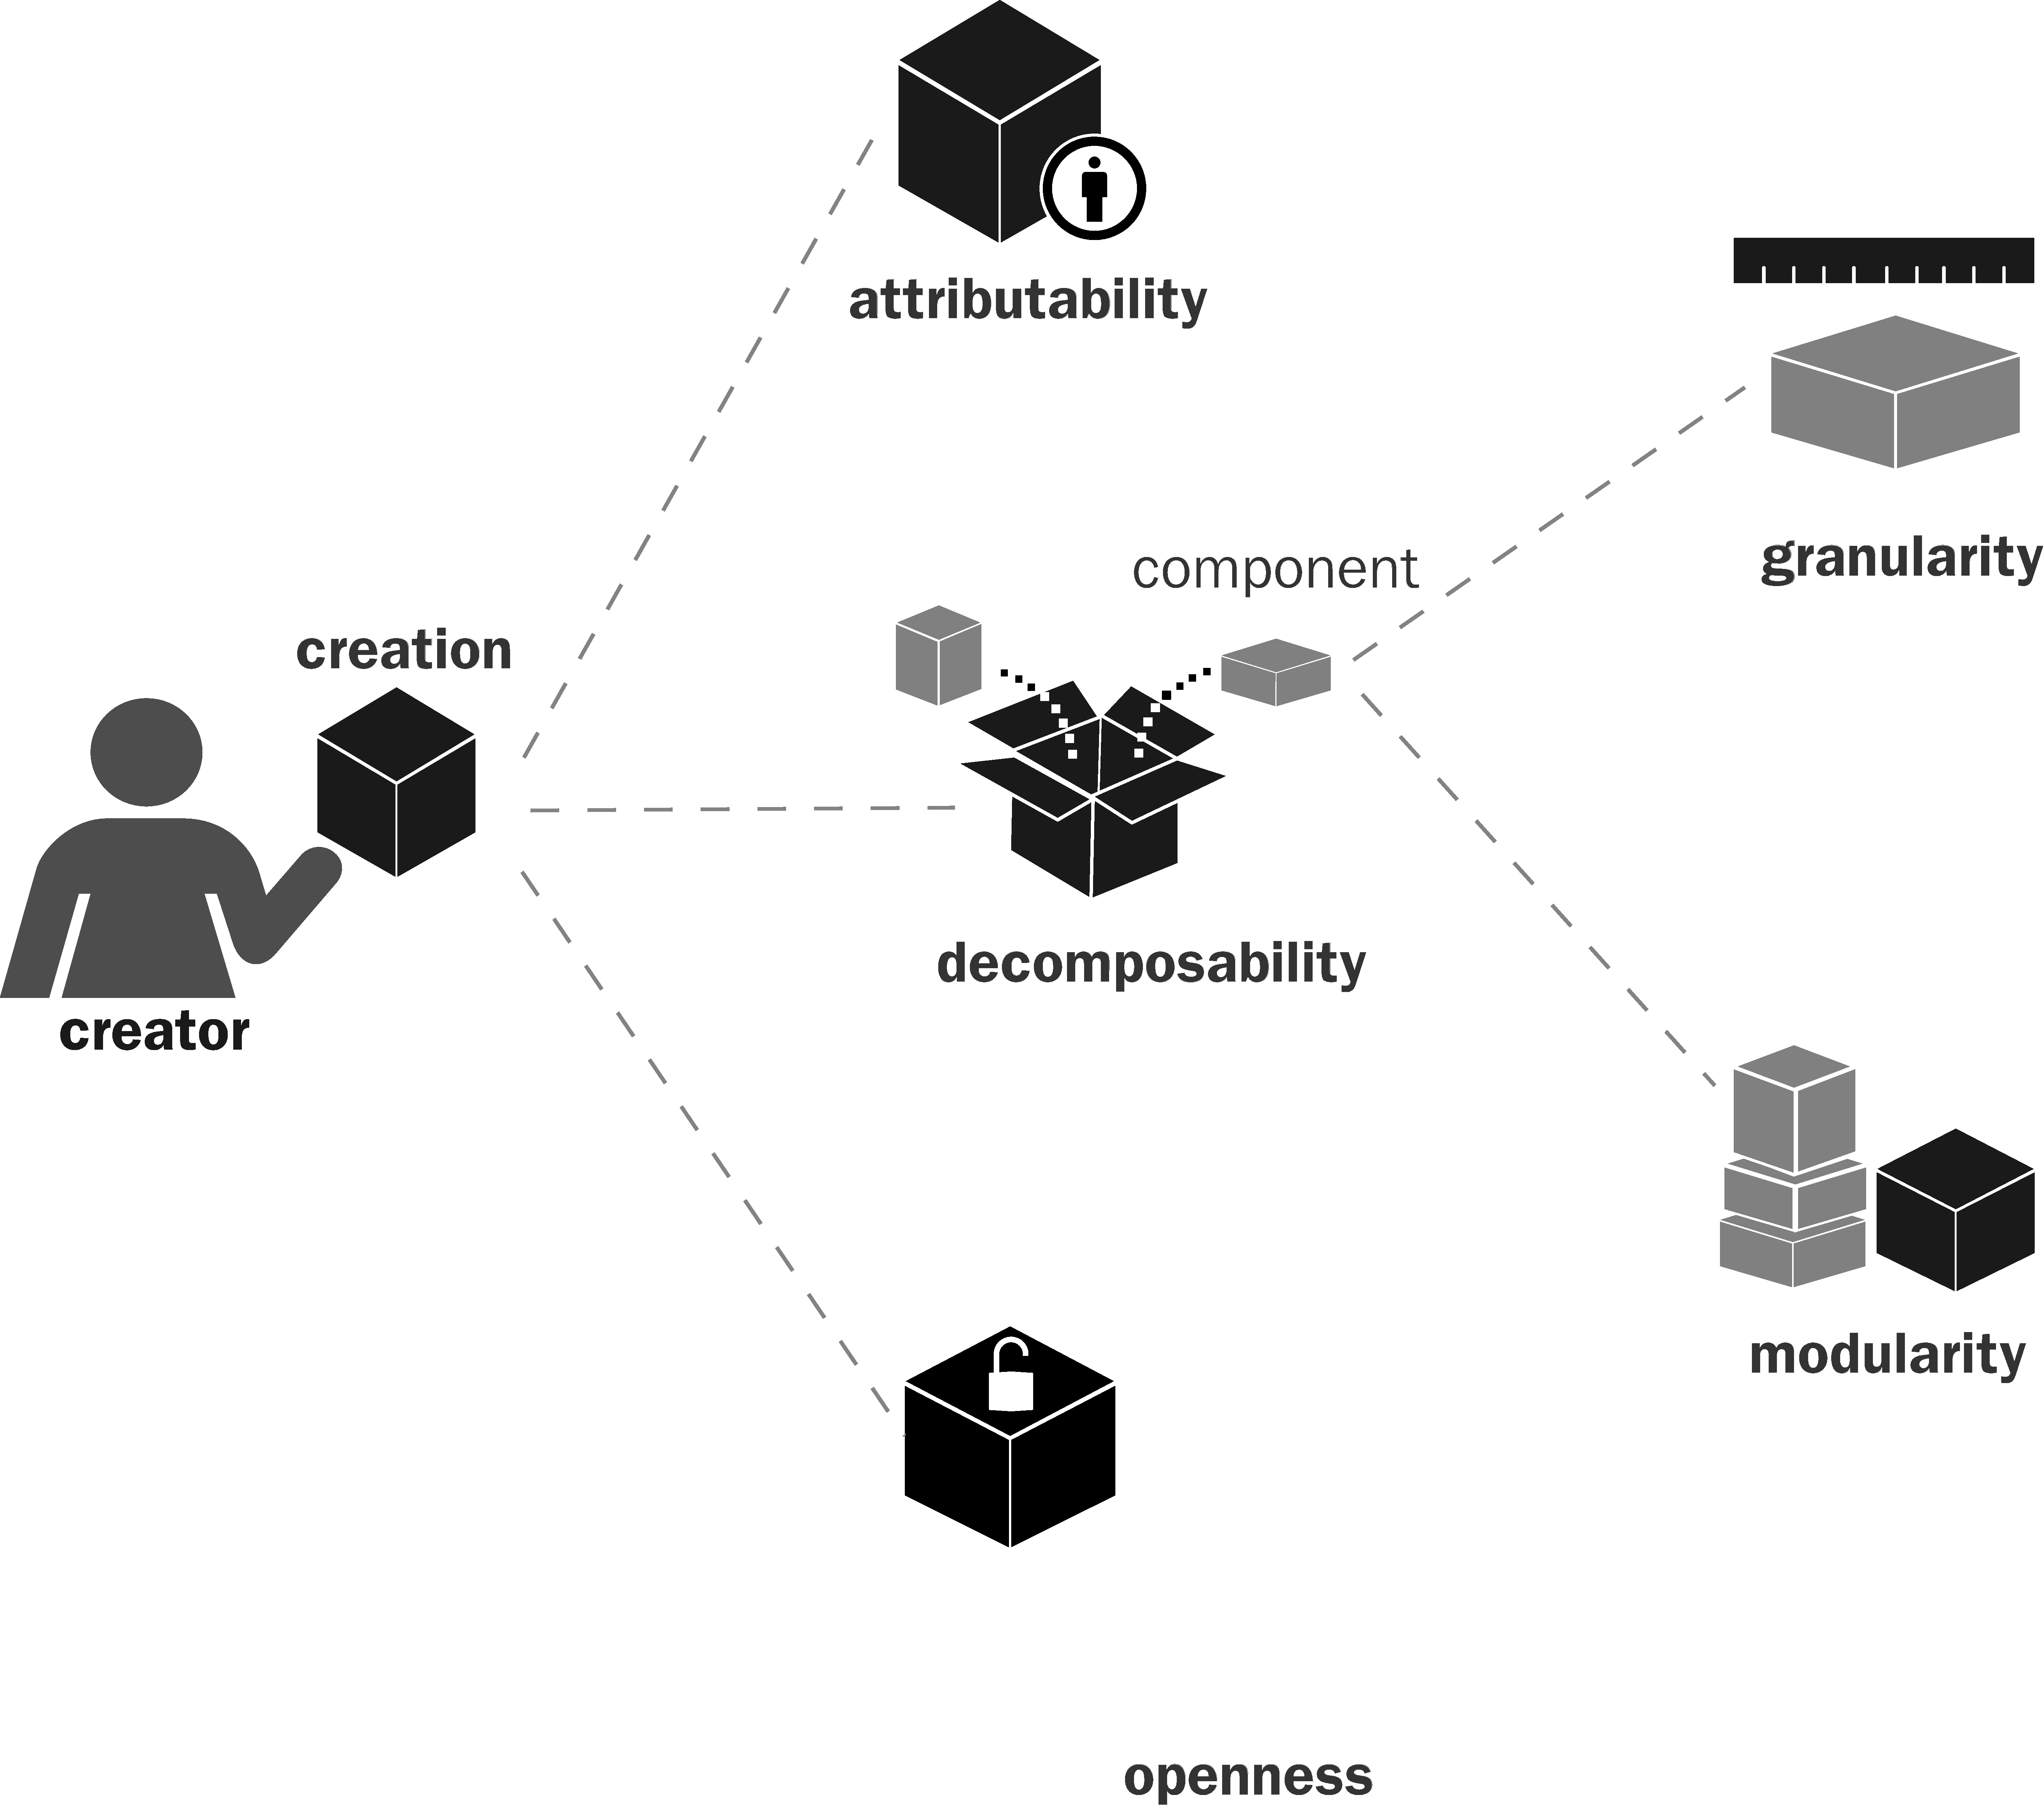
\includegraphics[width=3.25in]{figures/structure.pdf}
\caption{Structural dimensions of a remixing system}
\label{fig:structure}
\end{figure}

\subsection{Granularity}
Granularity is the size of projects' modules \citet{benkler_coases_2002}. 
In Scratch, projects have a couple levels of granularity.
Projects are made up of ``sprites'', for example, characters in a game or a elements in the user interface elements of an interact simulations.
Each sprite can have ``scripts'' or  stacks of programming blocks that control the sprite's behavior such as its position on the screen, its looks, sounds and interaction with other sprites and the user (via mouse, keyboard, or other sensors).
Each sprite also has one or more costumes or images that represent the different visual states of a sprite.
Sprites can also have sounds that are played programmatically, for example, a character in a game could make a sound each time it jumps.

\subsubsection{Proposed work}
The Scratch Online Community, by default it only allows for sharing at the coarsest degree of granularity: only projects can be shared. 
I plan to analyze the implications of this design decision and the ways  people get around the limitations of the architecture.

I have anectdotal evidence that Scratch participants get around the granularity limitations by sharing full projects with the sole intention of sharing a single sprite, script, image or sound.
This need for finer granularity often stems from a desire to engage in sharing practices that the original design did not anticipate. For example, I have documented before the existence of ``coloring contests'' \citep{nickerson_appropriation_2011} where Scratch community remix in order to add color to an image. or as part of group collaboration.
I plan to look these practices in more detail to understand the ways in which a finer granularity mechanisms would help support different types of creative and collaborative learning practices beyond the the existing research that suggests that finer granularity is correlated to the number of people engaged in cooperative activities.

In order to analyze the effect of explicitly supporting finer degree of granularity through a natural experiment, I plan to analyze the adoption ``Scratch Resources'' \footnote{Available at http://resources.scratchr.org}, a website created by members of the Scratch community to support sharing sprites, images and sounds. 
% TODO link to Von Hippel at al on user innovation

Some of my motivating questions are: 
how common is sharing and remixing across the different levels of granularity available (even if not explicitly supported)?
what are the types of participants and motivations for sharing finer grained components?
what role does granularity play in the likelihood of a project being remixed controlling for all other factors?
how do different levels of granularity impact the type and quality of remixes?
how do different levels of granularuty support different levels of familiarity with Scratch, that is, are novices more likely to rely on coarser granularity when engaging in remixing as a scaffolding mechanism?

\subsection{Modularity}
\citet{benkler_coases_2002} defines modularity as the ``property of a project referring to the extent to which it can be broken down into smaller components, or modules, that can be independently and asynchronously produced before they are assembled into a whole.''
For the purpose of this work, I will separate two different aspects of modularity:
1. The ease of \emph{integrating} such components into new creations or remixes.
2. The ease of \emph{decomposing} an existing project into smaller components, typically for the purpose of remixing.
In this section I plan to analyze the term ``modularity'' by focusing on the first aspect.
In the next section, I will focuson the second aspect under the term ``decomposability''.

\subsubsection{Proposed Work}
There are some components or projects that can be more easily integrated into new projects. 
One of the questions I am intersted in exploring is what makes some components more modular than others.

For example, an image generated programmatically might be harder to integrate than one in bitmap format. 
A module that representing a cultural icon, such as Mario\footnote{Mario is a character in a popular video game called Mario Bros. from Nintendo Inc.}, is perhaps easier to integrate into other projects than an image of a less well-known character.
However, there are situation when new subcultural icons emerge within the Scratch community.
For example, a character called Maki-Tak created by a community member from New Zealand started a whole genre of projects, called Takis.
These projects use adaptations of that lizard. 
% Other examples: Mr happy Man
There are also situations where some components are remixed despite their internal complexity which might indicate that these could be built in a way that their internal complexity is hidden and remixing them is easy. 
For example there is a sprite created by an advanced Scratch user that represented a physics simulation of a string. 
This project was later remixed in a project where it represented a necklace.

I plan to operationalize the assessment of modularity by measuring its adoption through number of remixes.
The assumption will be that more modular components are remixed more.
I will examine this in two types of components:  ``samples'' and ``community-generated''.
% Sample components are those that come pre-installed with Scratch. For example, sample images, sounds, sprites and projects in some cases.
% Community-generated are those created by end-users.
For example, ``jetpack girl'' is a sample script consisting of five costumes and  sounds for a flying character that can be controlled with the keyboard.
The code of the sprite comes with an invitation to remix: ``Import me into your own project'' and an explanation on how to use it ``arrow keys make me fly''.
These sample components are not only sprites, there are also hundreds of images and sounds that come with Scratch such as photos of people, animals, things, etc.
In addition to these sample components, there are thousands of components created by community members that are remixed and that can be found in places like Scratch Resources and Scratch projects that explicitly state that they include sprites, images and sounds for others to reuse.

The type of questions I will try to answer are then are:
1. What technical or cultural attributes are linked with component modularity? 
2. Are more modular components used more often by newcomers and do they provide scaffolding in their learning of Scratch programming?
3. Are community-generated components more often created by advanced users?

\subsection{Decomposability}
Building on the concept of modularity examined before, in this section I will examine decomposability as the ease of decomposing a compiled project.
Decomposability is the ease of breaking something apart for the purpose of remixing it.
Therefore decomposability depends on the internal complexity of a project, which in itself is dependent on the expertise of the person attempting to decompose the project.
For example, one can argue that images in Flickr.com are harder to decompose than those in OpenClipart.org, which provides the source vectors, or Aviary.com which provides the bitmap images that were used to create an image.
The same happens with software applications that provide the source code in contrast with thost that only provide the final compiled executable.
But even if the source is provided, there are some cases where projects are ``impenetrable'' due to their complexity or a missmatch between the expertise of the person trying to decompose a project and the complexity of the project. 
For example, for a novice programmer having access to the source code of the Linux kernel might not allow for easy decomposability.

In Scratch, all the sources of a project are provided so the decomposablity of a project depends, among other things, more on how interconnected its different components are. 
For example, sometimes sprites ``broadcast'' messages back and forth making their decomposablity much harder than those that are self-contained.
Also, some creators add instructions to their projects explaining how they can be broken apart, while others obfuscate their code to prevent remixing.

\subsubsection{Proposed Work}
I will first do a manual analysis of a sample projects to observe patterns of decomposability. 
Using the findings of this analysis I will come up with mechanisms to automate the evaluation of decomposability. 
For example, it is possible that a decomposability metric could depend on the use of particular blocks (the ``broadcast'' block could reduce its ranking, while comments in the code would increase it), explicit obfuscation or matching between the average expertise level of community members and the expertise required to understand a project.

I will also look at remixes to analyze how different they are from their original project. 
The assumption would be that ``impenetrable'' projects would be correlated with no remixing or to superficial remixes, such as slights changes in the images,
while highly decomposable projects are associated with significant differences betweent the remix and the original.

I will also analyze in detail the practices of code obfuscation and the strategies people use to discourage decomposability of their projects.

\subsection{Attributability}
Creators often want to get credit for their work. 
For example, the Creative Commons license originally had attribution as one of the options of their licenses but after analyzing several years of usage of the licenses they found that very few people waived the attribution clause. 
This led them to include attribution by default in all their licenses (and create a separate license for completely public domain works) \citep{brown_announcing_2004}
In order to further our understanding of attribution when desigining a remixing system it is important to know the role attribution plays in supporting cooperative behavior among members of a remxing online community.

In Scratch, we have run some design experiments playing with attribution. 
For example, we found evidence that suggests that about 20\% of creators object to seeing their projects remixed \citep{hill_responses_2010}.
We also have anectdotal evidence that people who objected to remixing of their project referred to lack of credit as one of the problems.
In order to address this,I added a mechanism that would automatically give credit to the creator of the original project whenever a remix was uploaded (e.g. ``Shared by John, based on Mary's project'').
Using that design intervention as a natural experiment, we found evidence that suggests that people not only want to get credit but that they prefer the credit given by another person over the automatic attribution given by the system \cite{monroy-hernandez_computers_2011}. 

\subsubsection{Proposed Work}
I plan to extend this work with additional experiments.
For example, one of the common complains against remixing is that the textual description of projects often gets copied from an original project onto its remixes.
This often gives the wrong impression that those notes were written by the remixer rather than the original creator.
I plan to add a mechanism to show a distinction between the notes written by the originator and those added by the remixer.
These additional notes will come with a mechanism to encourage remixers to explain the ways in which the original project was changed.
This will serve as a natural experiment to test out the additional value of not only giving binary representation of attribution but also give a qualifier explanation to the connection between a remix and the original project.

% TODO: Other experiments: 
% - Creator endorsed attribution.
% - Diff

\subsection{Openness}
Openness is not onl
% Across systems. Ethos explained. Creative commons version for kids. DeviatnArt conflicts
% 



I analyze the role remixing plays in participating in an online community of creators.
I look at how several forms of remixing (Figure~\ref{fig:function} are represented in the Scratch Online Community, how their use evolves, and how they do or do not support sociability and creative practices.
I analyze people's remixing behavior including their: 
1) modifying existing work, 
2) reusing components, 
3) collaborating with others in groups, 
4) persuading crowds to join remixing chains, 
5) inspiring others with ideas for new creations or 
6) self-appropriating their work to create something. 

\begin{figure}
\centering
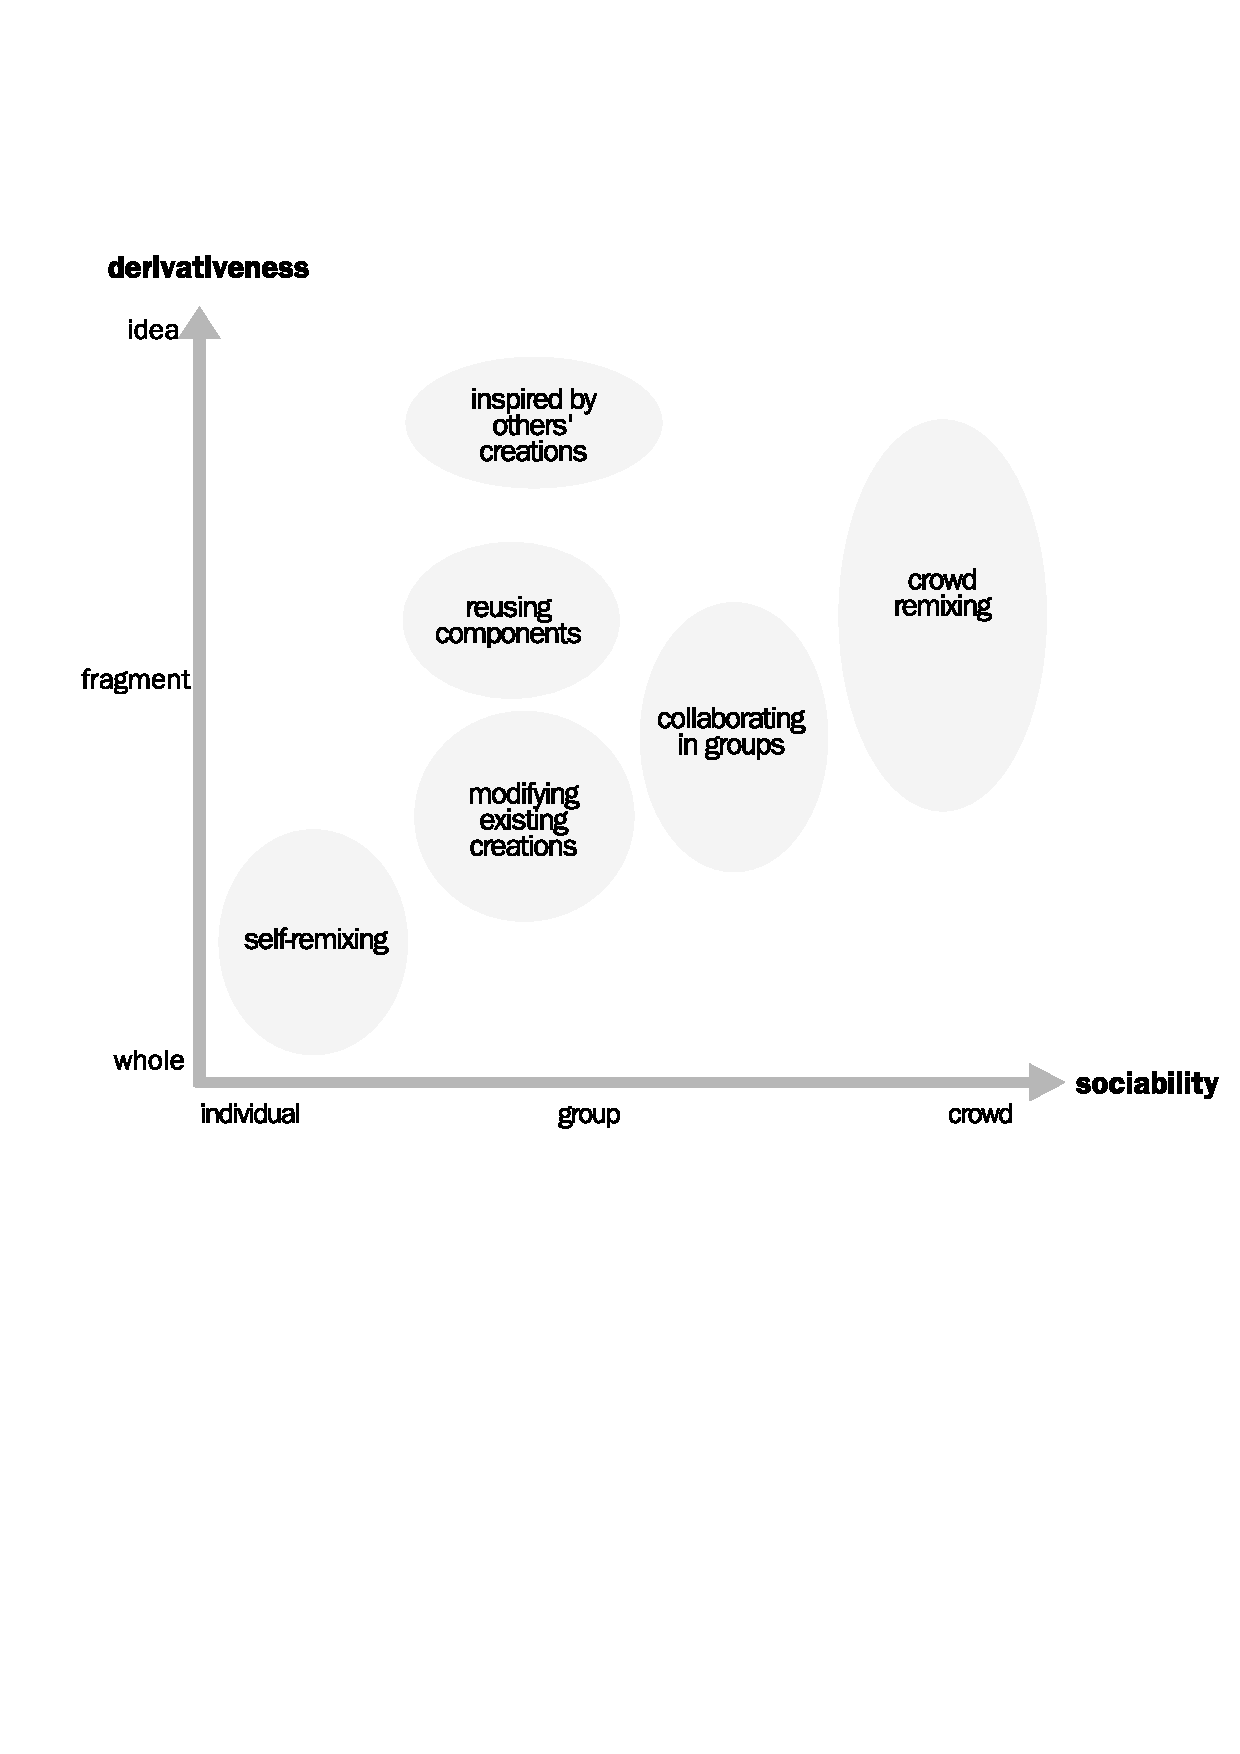
\includegraphics[width=3.25in]{figures/function.pdf}
\caption{Functional roles of remixing in the social and produc-focus dimensions}
\label{fig:function}
\end{figure}

% TODO:
% Proposed work:
% - Evolution of each type.
% - How do they engage in these different forms of production.
% - To what extent do these different forms of remixing support:
% a) scaffolding,  b) committment, c) creative and d) collaborative practices? e) reputation
% 	Look at people who get started by remixing and compare it to those who don't. Follow take other pats.
% 1. Modifying existing work. 
% 4. Crowds: coloring contests
% Some of these roles are analyzed from a network perspective. For example, the network of people engaged in colloring contests represents a group of people involved in a gift exchange network.


\subsection{Attitudes Toward Remixing}

I investigate remixers' and originators' attitudes toward remixing. In particular, I analyze how participants perceive remixing and how they do or do not cooperate by letting or encouraging others to reuse their work.
This analysis is driven by an interest in understanding how the system design may influence these attitudes. 
I plan to analyze these issues from the perspective of people whose projects are remixed as well as from those creating the remixes.
 
Previous work studying people's attitudes toward remixing in the Scratch Online Community \citep{hill_responses_2010, monroy-hernandez_computers_2011} found evidence that people are as likely to react negatively as they are to react positively when someone remixes their work. 
Additionally, we have found originators are more likely to respond negatively when their projects are more complex.

Broadly speaking, people whose projects are remixed react either by being indifferent to it, accepting it, conditionally accepting it (for example, specific rules or norms have to be followed), or by explicitly opposing to it (for example, posting a negative reaction comment like ``you stole my project!'').
Similarly, remixers go about remixing by either being oblivious of the norms (for example, giving credit or asking for permission has emerged as a norm in the  community), or cautiously doing it by asking for permission first, or even being confrontational and using remixing as a form of ``trolling'' \citep{donath_identity_1998}.

\subsubsection{Proposed Work}

I plan to analyze people's attitudes toward remixing in the Scratch Online Community through case studies and experiments.
Additionally, I expect these metrics of people's responses and attitudes will serve to understand the health of the community and to motivate further design interventions.
In particular, I propose two studies for studying Scratch participant's attitudes toward remixing that complement the two recently published articles \citep{monroy-hernandez_computers_2011,hill_responses_2010}.


% NOTES The overarching questions are: How do young people respond to remixing? How are these attitudes represented in the community? When do they embrace remixing and when do they reject it?  I have and will analyze young people’s attitudes based on their words (interviews) comments, reports (flags) and strategies for deterring (obfuscation, pseudo-licenses, Vigilantism) or supporting remixing (commenting, scaffolding, framework approach, creation of narratives).
% Crowding out remixing by featuring
% Evolution of reactions as design changes

\emph{Plasticity of Virtue.}
For the past five months, I have been running an experiment aimed at ascertaining how people's attitudes toward remixing could be changed through a design intervention.
The study consists of sending notification messages that try to appeal to various motivations for cooperating in the Scratch online community. 
As mentioned before, a contentious issue in the Scratch community has been the acceptance of remixing by those whose projects are remixed. 
People only learn about remixes of their projects by browsing their project pages and looking at the list of derivative works. 
The notification page is the principal form of communication between the system and the users.
The experiment consists of informing people when one of their projects gets remixed.
This experiment provides an opportunity to test: 1) the comparative effectiveness of various ways of communicating the same event and 2) the permanency of the behavioral change, if any. 

The experiment consists of two phases.
The first is the notification period. 
When someone's project gets remixed, the system automatically assigns the creator of that project to one of the treatment conditions. 
From then on, the person receives messages whenever someone remixes his or her project. The message depends on the treatment category.
For example some messages are neutral (for example, ``Your project FooBar was remixed. Check out the remix.''); 
others are positive (for example,``Congratulations! Your project FooBar was remixed. Check out the remix .'');
others try to elicit generosity (for example, ``Your project FooBar has been remixed. Sharing your work is a generous thing to do and a great thing for the Scratch community! Check out the remix.'').
Other messages try to elicit conformity, reputation building and fairness.
Finally, a control category is added where no notification is sent.

The second phase of the experiment is sending no notifications. In this phase of the experiment, the notifications stop and people's reactions continue to be logged.

After a few weeks we look at the results of pre- and post-phase one, to analyze the effectiveness of each treatment by measuring the number of positive and negative reactions that originators leave on the remixes. 
Additionally, I analyze the pre- and post-phase two, to see how malleable the behavior is.

\emph{Featuring Top Remixes.}
The home page of the Scratch website now has a section called ``What the Community is Remixing''  that features the three top remixed projects in the past two weeks.
This section did not exist when the website was first unveiled.
In fact, this section was added as measure to counter the backlash against remixing by showing that getting one's project remixed could increase social status in the community (being on the front page is an important reputation-building mechanism).
This study aims at assessing whether a design intervention aimed at increasing the acceptance of remixing had a ``crowding out'' effect by decreasing the quality or effort people put into making their remixes.
I have devised metrics to operationalize the complexity and effort a creator puts into creating his or her project. These metrics are based on the number of sprites, scripts, blocks, diversity of blocks and time it took from the first save to the hard disk until it gets shared on the website.




\chapter{Contributions}

Among the contributions of this thesis are:
\begin{itemize}
\item Conceptualization, design and implementation of a large online community of amateur creators.
\item Collection of a large corpus of research data that includes millions of interactive media projects and activity logs of more than half-a-million accounts.\footnote{Currently working on ways to release an anonymized version of these data to other researchers.}
\item A set of studies of sociotechnical design interventions.
\item A set of descriptive case studies of the activity on the Scratch Online Community.
\item A multidisciplinary framework to analyze and understand a new cultural phenomenon.
\end{itemize}

\chapter{Plan}

For the past four years, I have led the development of the Scratch website and worked on cultivating an online community that has grown to close to eight hundred thousand people.
I have also published work describing the ways people participate, create, collaborate and remix on the Scratch Online Community \citep{monroy-hernandez_scratchr:_2007, monroy-hernandez_empowering_2008, monroy-hernandez_computers_2011, hill_responses_2010, aragon_tale_2009, nickerson_appropriation_2011, brennan_making_2010}.

In this phase of my research, I plan to work towards analyzing in structural, functional and attitudinal aspects of remixing in Scratch to better understand this specific phenomenon as well as the community at large.
I plan to integrate the findings into a cohesive framework for understanding remixing in a way that can be generalizable.

\section{Resources}
The technical infrastructure to support the website is in already in place.
In the upcoming days, I am planning to add two extra servers that will help further scale the website to handle more traffic and that will let me analyze the large corpus of data.
We also have a community manager, an IT consultant and a database specialist on retainer who will be able to assist with this research.
I already have the necessary approvals from COUHES\footnote{Committee On the Use of Humans as Experimental Subjects}.

\section{Timeline}
\begin{itemize}
\item May 2011 -- Data aggregation. In the first month, I plan to put together the data sets necessary to answer some of the research questions described in this document. A lot of the data is already collected but it needs to be put together in an appropriate format for answering each question. This phase is also exploratory, which will help to tweak the framework in this proposal to better represent the patterns found in the data.
\item May 2011 -- Survey and experiment deployment. Also in the first month, I plan to deploy the necessary design interventions that will help get the necessary data that I do not have already. Most of these experiments are already programmed and just need to be tweaked.
\item June, July 2011 -- Data analysis. I plan to create the necessary visualizations and statistical analyses to examine some of the research questions outlined in this proposal. Additionally, I will build a set of representative case studies and execute the necessary interviews.
\item August 2011 -- Results. I plan to put together the findings in a structured form, and integrate all the findings into a cohesive document accessible to a broad audience.
\item September 2011 -- Draft. I will have a first full draft of my dissertation.
\item January 2012 -- Defense.
\item February 2012 -- Final version.
\end{itemize}

%Other chapters go here
%%Appendices
%\appendix
%Appendices go here. Structure is same as for other chapters
%%The bibliography
%\include{biblio}
\def\newblock{\hskip .11em plus .33em minus .07em}%not defined in the chi style
\bibliography{biblio}
\end{document}

%end file
